\documentclass[ignorenonframetext,]{beamer}
\setbeamertemplate{caption}[numbered]
\setbeamertemplate{caption label separator}{:}
\setbeamercolor{caption name}{fg=normal text.fg}
\usepackage{amssymb,amsmath}
\usepackage{ifxetex,ifluatex}
\usepackage{fixltx2e} % provides \textsubscript
\usepackage{lmodern}
\ifxetex
  \usepackage{fontspec,xltxtra,xunicode}
  \defaultfontfeatures{Mapping=tex-text,Scale=MatchLowercase}
  \newcommand{\euro}{€}
\else
  \ifluatex
    \usepackage{fontspec}
    \defaultfontfeatures{Mapping=tex-text,Scale=MatchLowercase}
    \newcommand{\euro}{€}
  \else
    \usepackage[T1]{fontenc}
    \usepackage[utf8]{inputenc}
      \fi
\fi
% use upquote if available, for straight quotes in verbatim environments
\IfFileExists{upquote.sty}{\usepackage{upquote}}{}
% use microtype if available
\IfFileExists{microtype.sty}{\usepackage{microtype}}{}
\usepackage{longtable,booktabs}
\usepackage{caption}
% These lines are needed to make table captions work with longtable:
\makeatletter
\def\fnum@table{\tablename~\thetable}
\makeatother
\usepackage{graphicx}
\makeatletter
\def\maxwidth{\ifdim\Gin@nat@width>\linewidth\linewidth\else\Gin@nat@width\fi}
\def\maxheight{\ifdim\Gin@nat@height>\textheight0.8\textheight\else\Gin@nat@height\fi}
\makeatother
% Scale images if necessary, so that they will not overflow the page
% margins by default, and it is still possible to overwrite the defaults
% using explicit options in \includegraphics[width, height, ...]{}
\setkeys{Gin}{width=\maxwidth,height=\maxheight,keepaspectratio}



\setlength{\parindent}{0pt}
\setlength{\parskip}{6pt plus 2pt minus 1pt}
\setlength{\emergencystretch}{3em}  % prevent overfull lines
\setcounter{secnumdepth}{0}

\usepackage{amsmath,verbatim}

\usepackage{fancyvrb}
\usepackage{manfnt}
\usepackage[normalem]{ulem}

%\usepackage[colorlinks=true]{hyperref}

\mode<presentation>{\usetheme{Malmoe}}

%\synctex=1

\setbeamertemplate{headline}{}


\setbeamerfont{footline}{size=\scriptsize}
\setbeamerfont{frametitle}{shape=\scshape}
\setbeamertemplate{itemize items}[circle]
\setbeamercovered{transparent}

\setbeamertemplate{navigation symbols}{}
\setbeamertemplate{footline}[frame number]{} 


\definecolor{forest}{rgb}{0, .5, 0}
\definecolor{brick}{rgb}{.5, 0, 0}
\definecolor{darkgreen}{rgb}{0, .5, 0}
\definecolor{darkred}{rgb}{.7, .15, .15}
\definecolor{darkblue}{rgb}{0, 0, .5}
\definecolor{Green}{rgb}{0.2,1,0.2}


\newcommand{\R}{\textsf{R}}
\newcommand{\RStudio}{\textsl{R Studio}}


\usepackage[english]{babel}
%\usepackage{palatino}
\usepackage[T1]{fontenc}


% make all tt fonts bold to look more like Verbatim
\usepackage{lmodern}
\renewcommand\ttfamily{\usefont{T1}{lmtt}{m}{n}}

% Comment these out if you don't want a slide with just the
% part/section/subsection/subsubsection title:
\AtBeginPart{
  \let\insertpartnumber\relax
  \let\partname\relax
  \frame{\partpage}
}
\AtBeginSection{
  \let\insertsectionnumber\relax
 \let\sectionname\relax
 \frame{\sectionpage}
}
\AtBeginSubsection{
  \let\insertsubsectionnumber\relax
  \let\subsectionname\relax
  \frame{\subsectionpage}
}

\title{Statistics and the Medical Literature}
\author{Dave Harrington}
\date{September 12 \& 19, 2016}

\begin{document}
\frame{\titlepage}

\begin{frame}
\tableofcontents[hideallsubsections]
\end{frame}

\section{General remarks}\label{general-remarks}

\begin{frame}{Questions received so far}

\textit{Ike Swetlitz:}

How important is effect size when determining whether to publish, as
opposed to (or in addition to) statistical significance?

\begin{itemize}
\itemsep1pt\parskip0pt\parsep0pt
\item
  Very, but important effect sizes vary with disease, type of study
\end{itemize}

What do we look for in the power of a study?

\begin{itemize}
\itemsep1pt\parskip0pt\parsep0pt
\item
  Generally want it the power (probability of detecting important
  effect) \(\ge 80\%\)
\end{itemize}

Do we have standards for minimizing false positive and false negative
results?

\begin{itemize}
\item
  Yes, but they may vary with type of studies.
\item
  Generally false positive rate should be \(<5\%\)
\item
  False negative rate should be \(<20\%\)
\end{itemize}

\end{frame}

\begin{frame}{Questions}

\textit{Sharon Begley:}

How do we tell if a study is sufficiently powered to determine important
effect sizes?

\begin{itemize}
\item
  \normalsize{Design before study execution, confidence intervals after study is completed}
\item
  Is it possible to examine power as a function of effect size?

  \begin{itemize}
  \itemsep1pt\parskip0pt\parsep0pt
  \item
    \normalsize{Yes, but should be done before study is launched}
  \end{itemize}
\item
  How to interpret dropouts?

  \begin{itemize}
  \itemsep1pt\parskip0pt\parsep0pt
  \item
    \normalsize{With difficulty \ldots}
  \end{itemize}
\end{itemize}

\end{frame}

\begin{frame}{What does a statistical reviewer look for?}

We do not expect designs or analyses to be perfect \medskip

We look for

\begin{itemize}
\item
  Accuracy, but this is difficult to check in detail in almost all
  cases.
\item
  Transparency
\item
  Following principles of scientific investigations: formulating a
  hypothesis, then testing it
\item
  Use of `state of the practice' methods
\item
  Sensitivity analyses: do different approaches lead to the same
  qualitative conclusion
\end{itemize}

\end{frame}

\begin{frame}{Statistical review at NEJM}

5 statistical reviewers, spanning range of subject areas \medskip  

We participate in the weekly AE sessions where papers are chosen for a
closer look.\medskip

We provide a detailed statistical review for any paper that the
associate editors wish to evaluate further.

\begin{itemize}
\item
  We guarantee a review in 2 weeks for routine papers
\item
  6 calendar days for fast track papers.
\end{itemize}

Approximately 15 - 20\% of papers are rejected on statistical grounds

\begin{itemize}
\itemsep1pt\parskip0pt\parsep0pt
\item
  But our focus is on trying to improve the statistics (if needed) in
  papers with strong science.
\end{itemize}

\end{frame}

\begin{frame}{Overview}

Techniques of statistics designed to

\begin{itemize}
\item
  `Minimize' the chance of a false positive (but it can never be 0)
\item
  `Maximize the chance of a true positive (but it can never be 1)
\item
  Acknowledge uncertainty in results, conclusions
\end{itemize}

Techniques and theory developed for settings much simpler than studies
with human subjects and with far less `noise'. \medskip

Considerable progress over the last 25 years, but methods for
interpreting large, complex studies still less than perfect

\begin{itemize}
\item
  Design sometimes requires compromise
\item
  Interpretation requires judgment
\end{itemize}

\end{frame}

\section{Interpreting the design}\label{interpreting-the-design}

\begin{frame}{Main elements of the design -- RCTs and observational
studies}

Plan to minimize bias?

\begin{itemize}
\item
  RCT: Randomization, blinding, identical evaluation/follow-up schedules
\item
  Observational studies: record important confounders, plan for post-hoc
  adjustment, perhaps include matching in recruitment
\end{itemize}

Chance of detecting important effects/associations? (Adequately powered,
at leat 80\%) \medskip

Plan to minimize false positive results if many endpoints/subgroups
examined?

\begin{itemize}
\itemsep1pt\parskip0pt\parsep0pt
\item
  More difficult with large observational studies, especially
  genomics/genetics
\end{itemize}

\end{frame}

\begin{frame}{Power and type I error}

Type I error (alpha error)

\begin{itemize}
\item
  Probability that trial will report a false positive, i.e., claim a
  significant result when there is no treatment effect.
\item
  Typically set no larger than 5\%
\item
  Depends on method of analysis, does not depend on sample size
\end{itemize}

Power

\begin{itemize}
\item
  Probability that the trial will report a true positive, i.e., claim a
  significant result when there is a treatment effect.
\item
  Should be 80\% or greater
\item
  Depends on sample size, method of analysis and size of treatment
  effect.
\item
  Power calculations relevant when study is designed.
\item
  Power calculations have little value after a study is complete.

  \begin{itemize}
  \itemsep1pt\parskip0pt\parsep0pt
  \item
    Precision measured through confidence intervals
  \end{itemize}
\end{itemize}

\end{frame}

\begin{frame}{Design of SPRINT}

From the methods section of the paper:

\begin{quote}
We planned a 2-year recruitment period, with a maximum follow-up of 6 years, and anticipated a loss to follow-up of 2\% per year. With an enrollment target of 9250 participants, we estimated  that the trial would have 88.7\% power to detect  a 20\% effect with respect to the primary outcome, assuming an event rate of 2.2\% in the standard-treatment group.
\end{quote}

\end{frame}

\begin{frame}{Calculating Power}

Next two slides show graphs of power in hypothetical study of blood
pressure lowering med. \medskip

Two medications, experimental vs control, using \(\alpha = 0.05\)

\begin{itemize}
\item
  First, power as a function of sample size if true effect is 3mmHg
  reduction
\item
  Second, power as a function of reduction in bp (effect size) for
  sample size 250 per group.
\end{itemize}

\end{frame}

\begin{frame}{Power vs.~sample size}

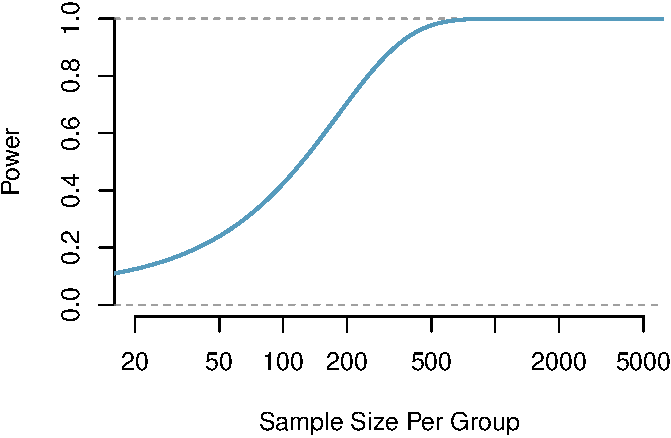
\includegraphics{reporter_course_harrington_files/figure-beamer/power_sample-1.pdf}\\
More than about 250 to 350 per group doesn't provide much additional
value.

\end{frame}

\begin{frame}{Power vs.~effect size, 250 participants per group}

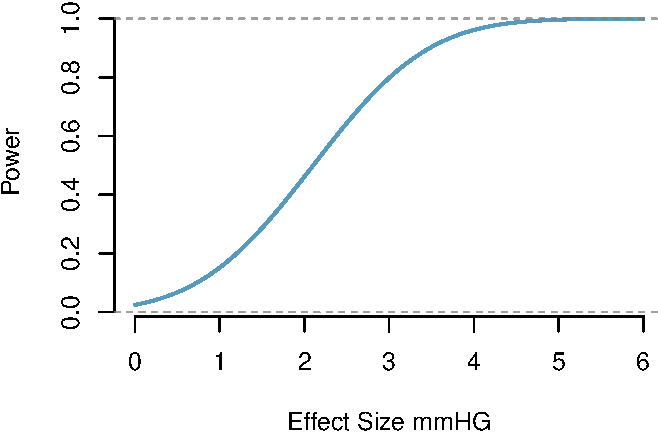
\includegraphics{reporter_course_harrington_files/figure-beamer/power_effect-1.pdf}\\

\end{frame}

\begin{frame}{Confidence intervals}

Confidence intervals are the preferred way to summarize outcome data.
\medskip

Easiest definition:

\begin{itemize}
\item
  Confidence interval provides a single estimate with a `margin of
  error'.
\item
  The size of the margin is determined by the variability in the data
  and the `confidence coefficient'

  \begin{itemize}
  \item
    Confidence coefficient is an estimate of the likelihood that the
    interval is correct
  \item
    95\% is typically used for confidence coefficient
  \end{itemize}
\end{itemize}

\end{frame}

\begin{frame}{Measuring precision after study completion}

From
\textit{Postmenopausal estrogen use and progestin use and the risk of cardiovascular disease,}
NEJM 15 August 1996

\begin{quote}
We observed a marked decrease in the risk of major coronary heart disease among women who took estrogen with progestin, as compared with the risk among women who did not use hormones (multivariate adjusted relative risk, 0.39; 95 percent confidence interval, 0.19 to 0.78) \ldots

\end{quote}

\end{frame}

\begin{frame}{Measuring precision after study completion}

\begin{quote}
However, there was no significant association between stroke and use of combined hormones (multivariate adjusted relative risk, 1.09; 95 percent confidence interval, 0.66 to 1.80) \ldots

\end{quote}

\end{frame}

\begin{frame}{Controlling type I error}

The more tests one does, the more likely it is that at least one will be
a false positive. \medskip

Suppose each test is done at level \(\alpha = 0.05\).

\begin{longtable}[c]{@{}cc@{}}
\toprule
\begin{minipage}[b]{0.34\columnwidth}\centering\strut
Number of Comparisons
\strut\end{minipage} &
\begin{minipage}[b]{0.38\columnwidth}\centering\strut
Experimentwise Error
\strut\end{minipage}\tabularnewline
\midrule
\endhead
\begin{minipage}[t]{0.34\columnwidth}\centering\strut
1
\strut\end{minipage} &
\begin{minipage}[t]{0.38\columnwidth}\centering\strut
0.05
\strut\end{minipage}\tabularnewline
\begin{minipage}[t]{0.34\columnwidth}\centering\strut
2
\strut\end{minipage} &
\begin{minipage}[t]{0.38\columnwidth}\centering\strut
0.10
\strut\end{minipage}\tabularnewline
\begin{minipage}[t]{0.34\columnwidth}\centering\strut
3
\strut\end{minipage} &
\begin{minipage}[t]{0.38\columnwidth}\centering\strut
0.14
\strut\end{minipage}\tabularnewline
\begin{minipage}[t]{0.34\columnwidth}\centering\strut
5
\strut\end{minipage} &
\begin{minipage}[t]{0.38\columnwidth}\centering\strut
0.23
\strut\end{minipage}\tabularnewline
\begin{minipage}[t]{0.34\columnwidth}\centering\strut
10
\strut\end{minipage} &
\begin{minipage}[t]{0.38\columnwidth}\centering\strut
0.40
\strut\end{minipage}\tabularnewline
\begin{minipage}[t]{0.34\columnwidth}\centering\strut
100
\strut\end{minipage} &
\begin{minipage}[t]{0.38\columnwidth}\centering\strut
\textgreater{}0.90
\strut\end{minipage}\tabularnewline
\bottomrule
\end{longtable}

\end{frame}

\begin{frame}{Are fMRI results reliable?}

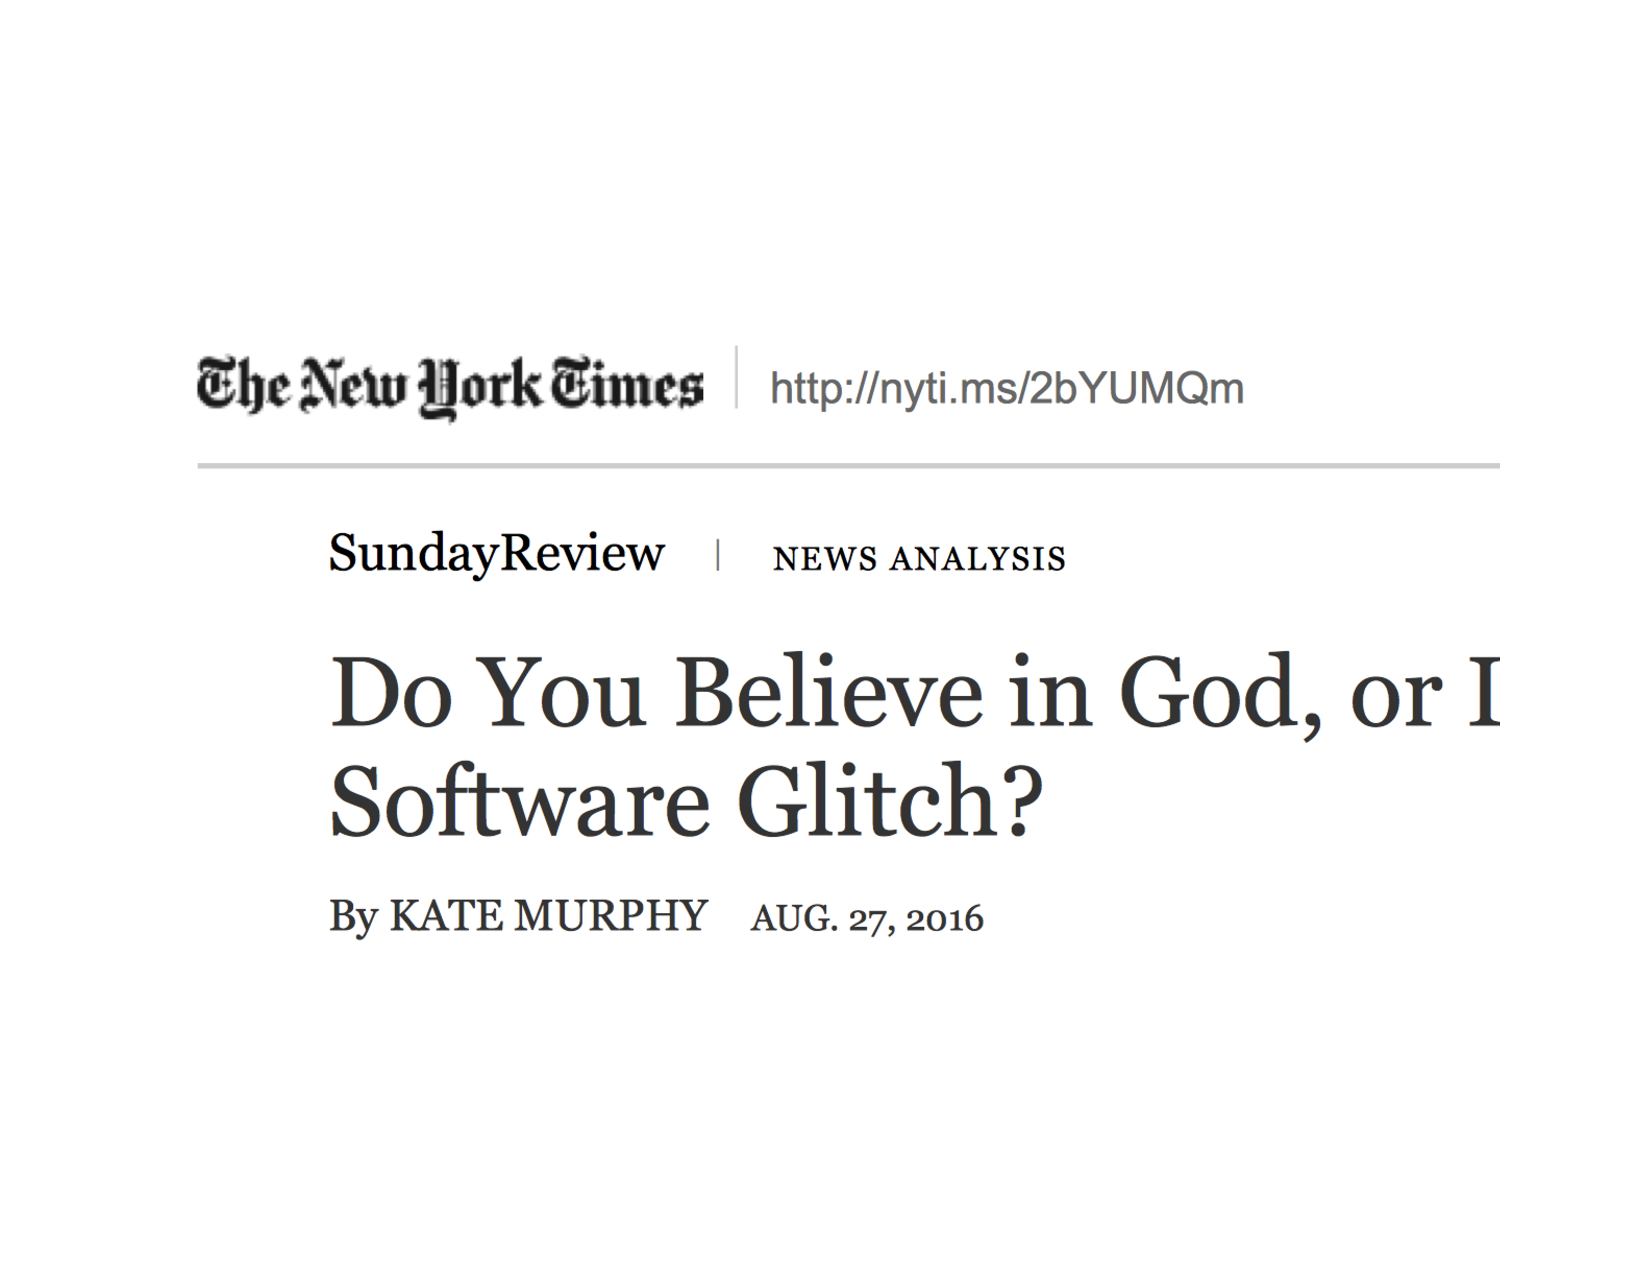
\includegraphics{figures/fmri_errors_2.pdf}

\end{frame}

\begin{frame}{Controlling type 1 error}

Assume target experimentwise error 5\% (\(\alpha =0.05\)) \medskip

Bonferroni approximation, no order specified for comparisons

\begin{itemize}
\item
  Divide significance level by number of planned tests
\item
  5 comparisons, use p = 0.01
\item
  Not practical when many comparisons planned, especially in genetics
  studies
\end{itemize}

\end{frame}

\begin{frame}{Controlling type 1 error\ldots}

Holm's method, no order specified

\begin{itemize}
\item
  Order the p-values from smallest to largest
\item
  Stop testing as soon as a p-value is too large
\item
  5 comparisons:

  \begin{itemize}
  \item
    Compare smallest p-value to 0.05/5 = 0.01.
  \item
    Compare next smallest to 0.05/4 = 0.0125.
  \item
    Next smallest to 0.05/3
  \item
    etc
  \end{itemize}
\end{itemize}

\end{frame}

\begin{frame}{Controlling type 1 error\ldots{}}

Holm-Bonferroni: one primary and several secondary endpoints

\begin{itemize}
\item
  Test primary outcome at \(\alpha = 0.05\). Stop testing if not
  significant
\item
  If significant, test secondary outcomes using Holm's method
\end{itemize}

The most important detail is sometimes hidden

\begin{itemize}
\itemsep1pt\parskip0pt\parsep0pt
\item
  Was the number of comparisons planned or reported the same as the
  number done?
\end{itemize}

\end{frame}

\begin{frame}{Anticipating many tests: Duty Hours}

NEJM 25 Feb 2016

\begin{quote}
Because one midpoint interim analysis was performed for data and safety monitoring purposes, the level of statistical significance for our final analyses of only patient outcomes was adjusted to 0.04 in order to maintain an overall significance level for the entire trial of 0.05. 
\end{quote}

\end{frame}

\begin{frame}{Duty hours \ldots}

\begin{quote}
In the context of a hypothesis of no difference [non-inferiority] in outcomes across study groups, correction for multiple comparisons was not a conservative approach for reducing the false discovery rate; thus, we report non–Bonferroni-corrected P values for all estimates. Bonferroni adjustment of P values for patient outcomes entails lowering the value from 0.04 to 0.004 (adjustment for 11 tests), whereas adjustment of P values for resident outcomes entails lowering the value from 0.05 to 0.0015 (adjustment for 34 tests).
\end{quote}

\end{frame}

\begin{frame}{Controlling type 1 error in genomic studies}

Genomic studies typically look at associations between a characteristic
and thousands of genes.

Two common methods:

\begin{itemize}
\item
  Use \(\alpha = 0.0000001\), or smaller.
\item
  Set an acceptable threshold for the proportion of discoveries that
  will be false, called the false discovery rate (FDR).

  \begin{itemize}
  \item
    Use sophisticated methods to estimate FDR, then keep it in bounds.
  \item
    Not discussed in these slides
  \end{itemize}
\end{itemize}

\end{frame}

\begin{frame}{Special topic: Non-inferiority (NI) randomized trials}

The NI design has one explicit and one implicit goal.

\begin{itemize}
\item
  Explicit goal: demonstrate that experimental treatment \(T\) is as
  effective, or nearly as effective, as best available therapy, C.
\item
  Implicit goal: demonstrate that \(T\) is better than placebo or no
  treatment (labeled \(P\) for placebo).
\end{itemize}

Ordinarily, both must be true for \(T\) to be a therapeutic option.

\end{frame}

\begin{frame}{Goals of NI Designs}

The ideal study design would be a three-arm design, with \(P\), \(C\),
and \(T\). \medskip

But a placebo or no treatment arm is usually unethical \medskip

The non-inferiority trial provides a direct comparison of \(T\) to
\(C\), but it does not provide a direct comparison of \(T\) to \(P\).

\end{frame}

\begin{frame}{NI designs}

The role of null and alternative hypotheses are reversed in NI trials.

Suppose on relative risk scale, the hazard ratio of Treatment vs control
should be no larger than 1.20

\begin{itemize}
\item
  1.20 is an example of a non-inferiority margin
\item
  The null hypothesis (\(H_0\)) is: Relative Risk \(\ge 1.20\)
\item
  The alternative hypothesis (\(H_A\)) is: Relative Risk \(< 1.20\)
\end{itemize}

Small \(p\)-values lead to rejection of \(H_0\)

\end{frame}

\begin{frame}{}

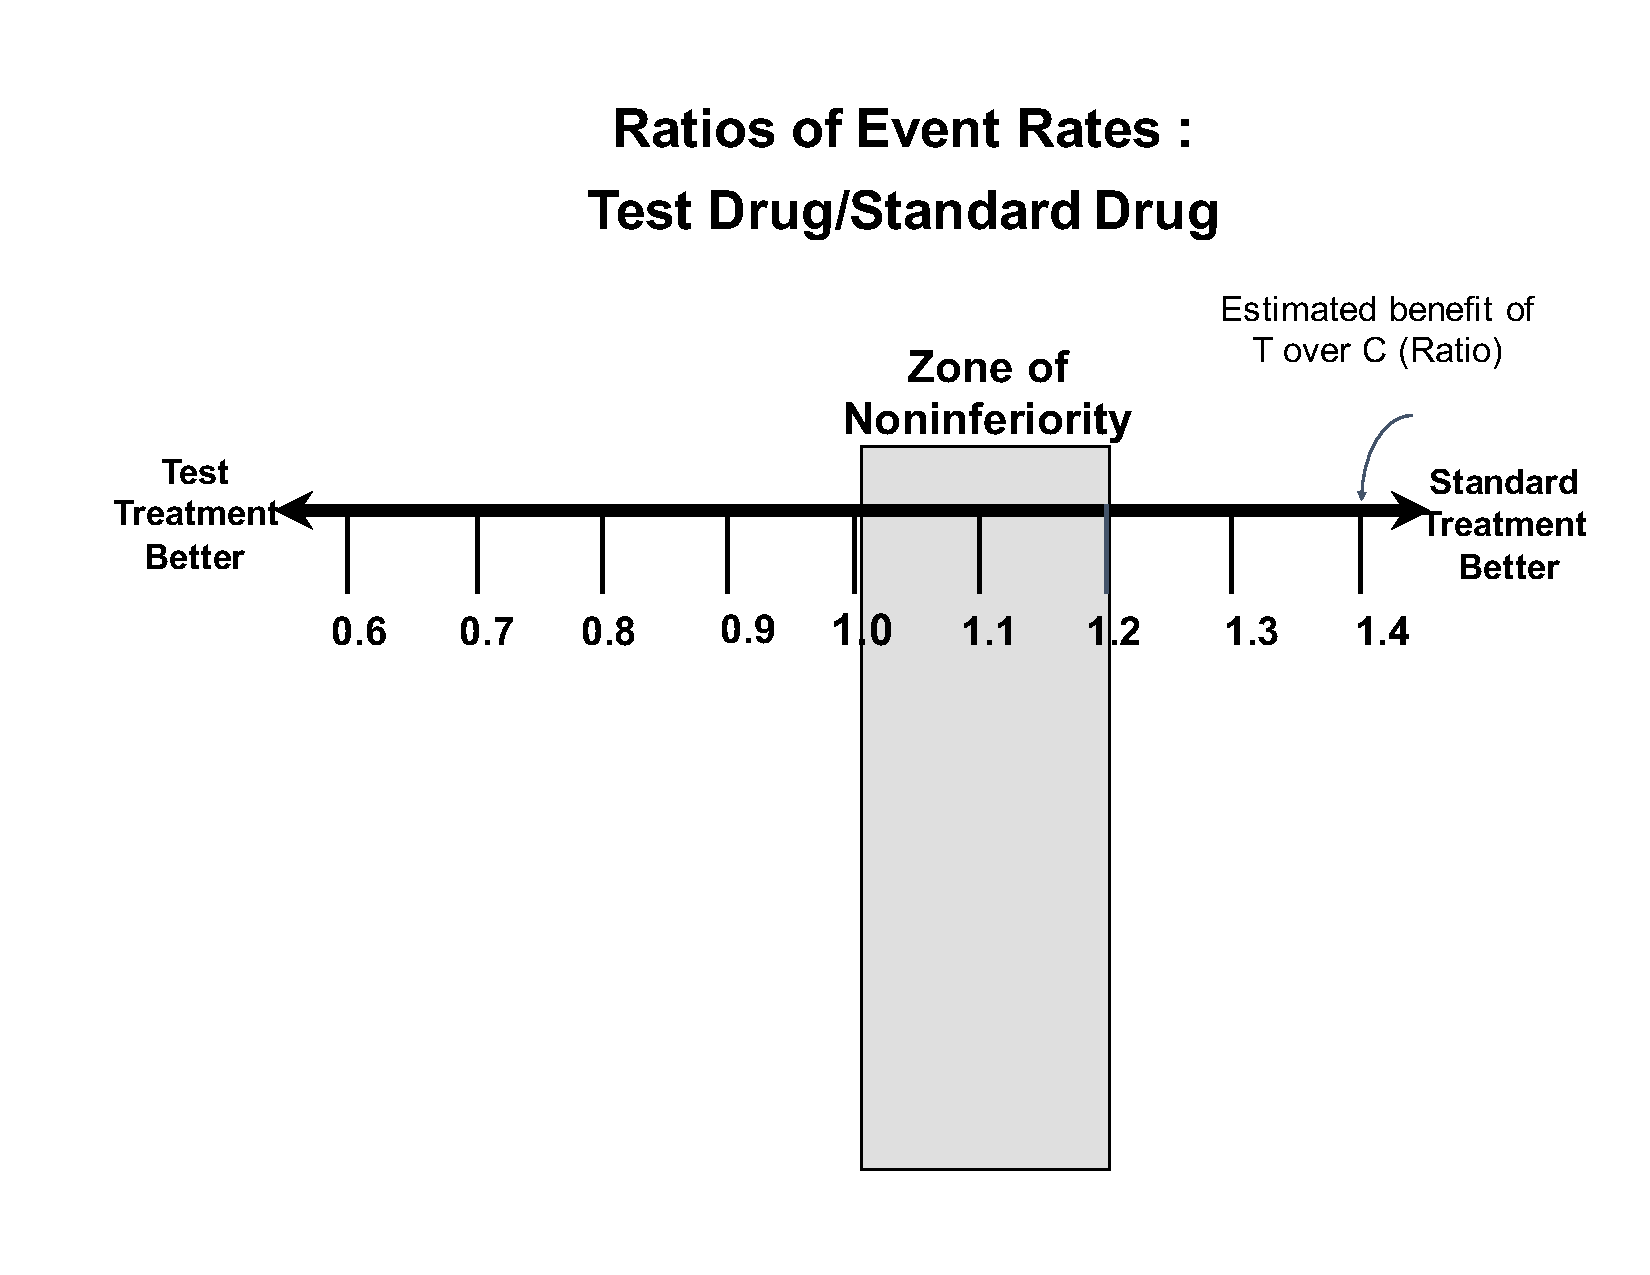
\includegraphics{figures/ni_ci_rr_empty.pdf}

\end{frame}

\begin{frame}{}

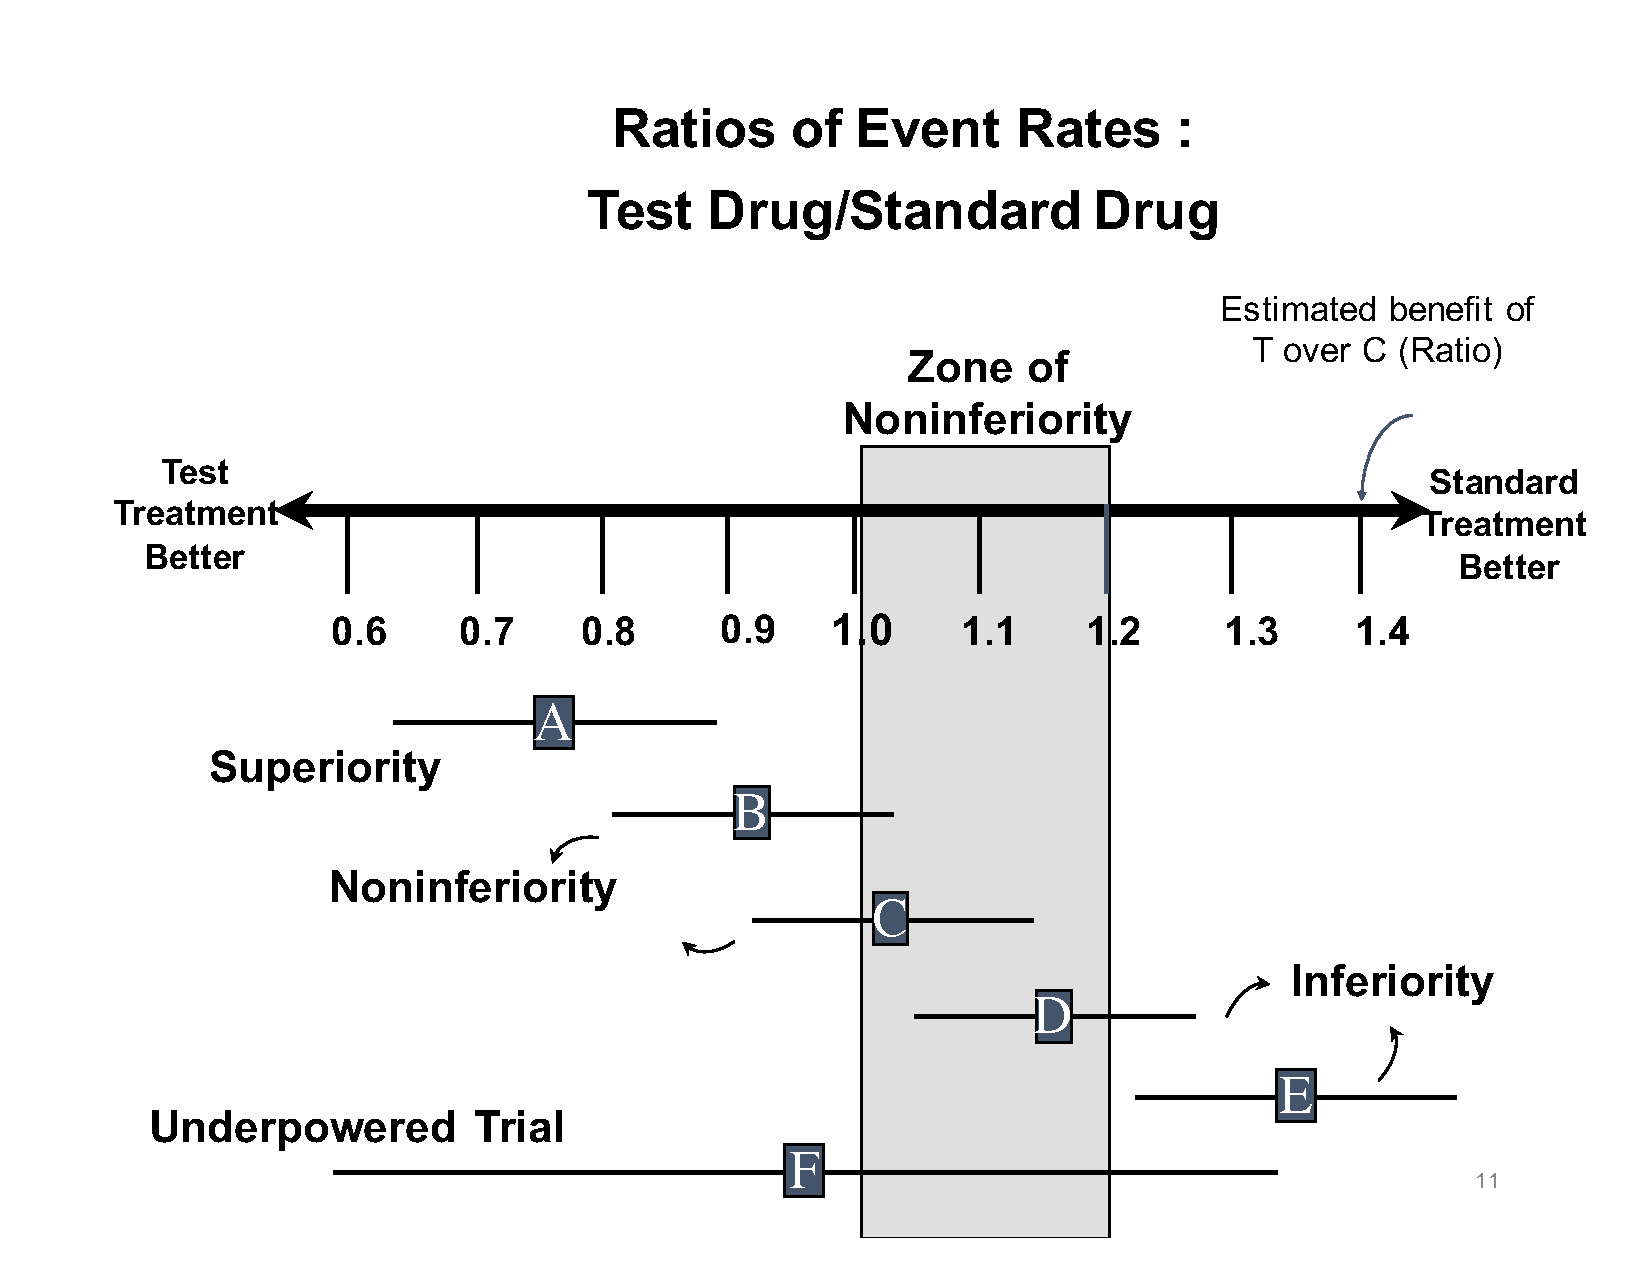
\includegraphics{figures/ni_ci_rr_full.pdf}

\end{frame}

\begin{frame}{}

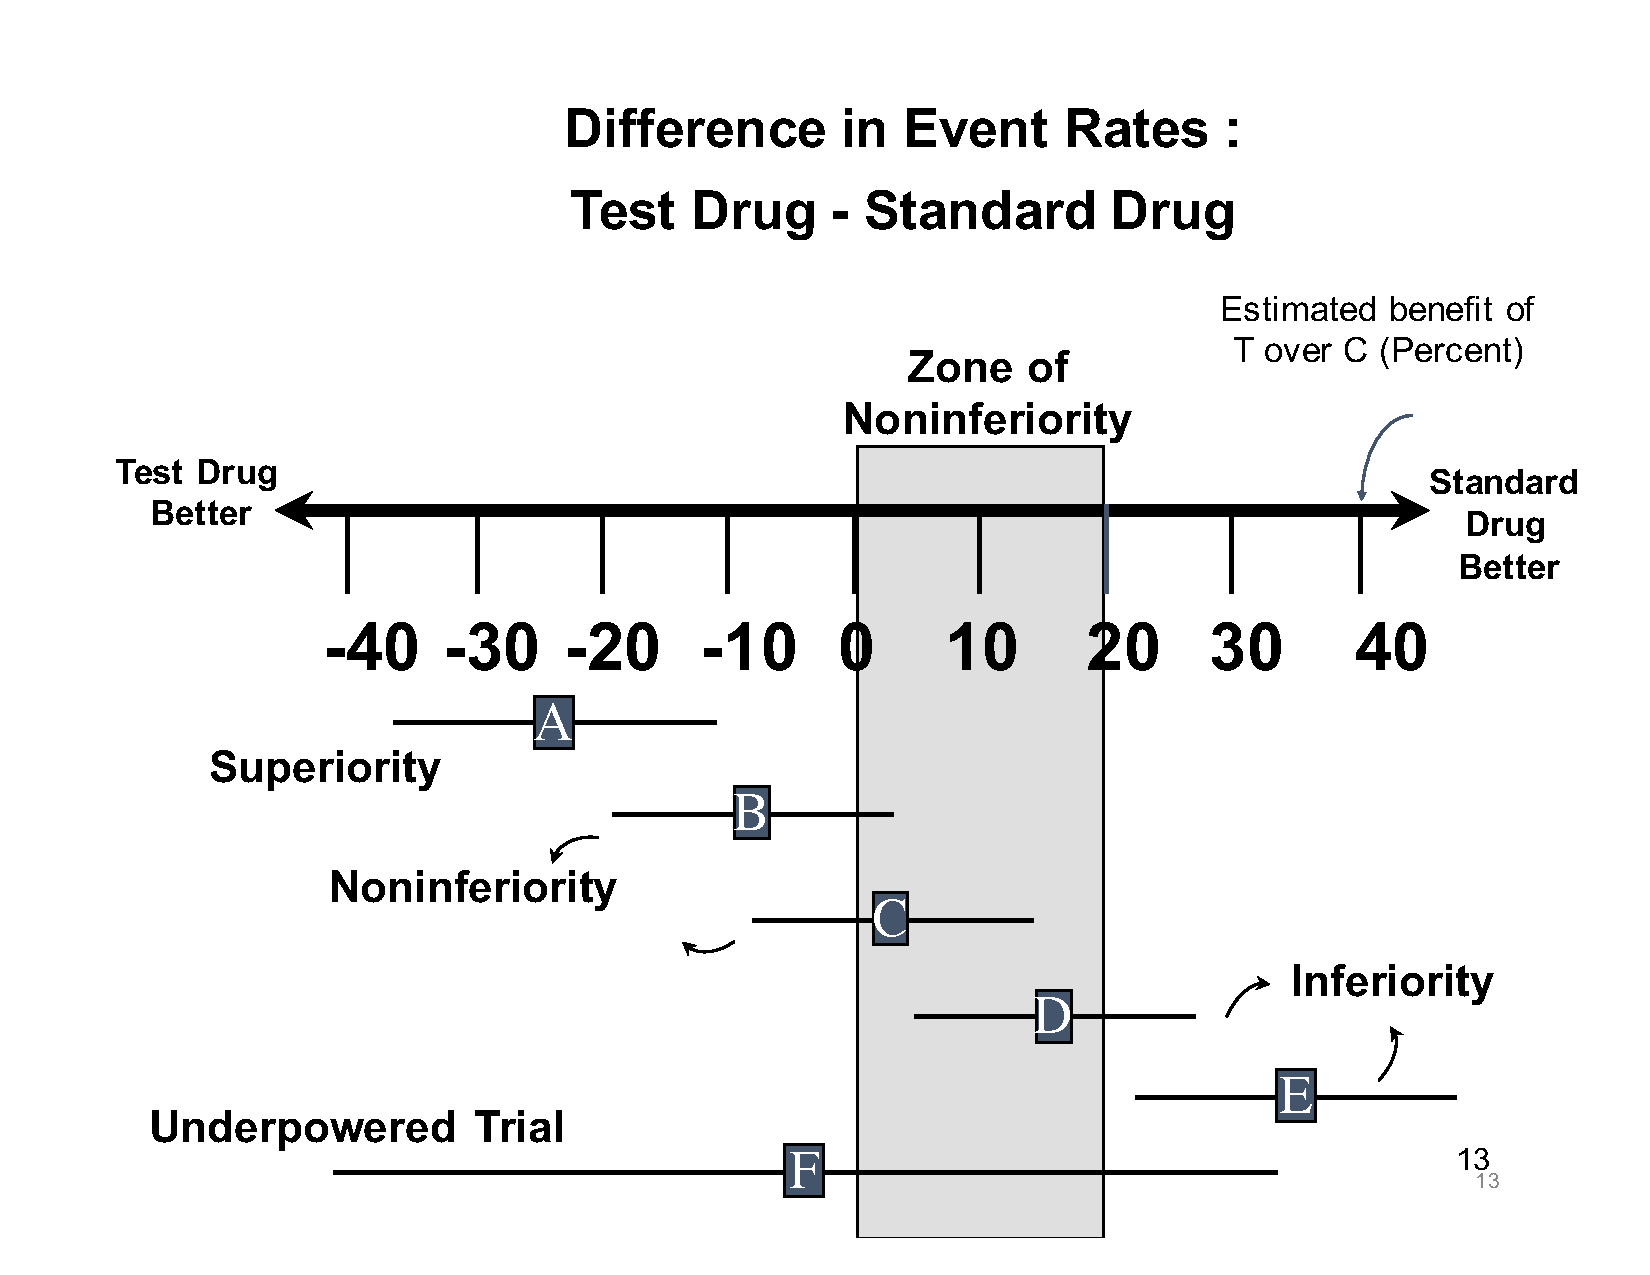
\includegraphics{figures/ni_ci_diff.pdf}

\end{frame}

\begin{frame}{Threats to Validity of NI Designs}

Non-inferiority designs have some intrinsic limitations that make them
more difficult to design and more vulnerable to problems than the
superiority design. \medskip

The following are the most important issues:

\begin{itemize}
\item
  Assay Sensitivity: possibility that \(T\) and \(C\) are ineffective,
  possibly from lack of adherence
\item
  Assay Constancy: \(C\) is still as effective as in historical trials
\item
  Dropouts can make two treatments seem more similar than they are.
\end{itemize}

\end{frame}

\section{Some Questions \ldots}\label{some-questions}

\begin{frame}{Explaining false positives}

Denise G asked for clarification on how false positives arise when
looking at several endpoints.

Here is a different explanation than the one I gave last week

\begin{itemize}
\item
  \(p\)-values are calculated assuming null hypothesis is true, i.e., no
  treatment effect.
\item
  Setting a \(p\)-value threshhold of 0.05 (the type I error) means that
  5\% of the time, a p-value will be significant when there is no
  treatment effect.
\item
  Extreme example: if one examines 100 subgroups, 5 of 100 comparisons
  (5\%) will be significant even when there is no treatment effect on
  any subgroups.
\item
  So a chance spruious finding will be very high.
\end{itemize}

\end{frame}

\begin{frame}{Propensity scores}

Best explained verbally, with reference to the example of confounding
found later in these slides.

\end{frame}

\section{Important issues in an
analysis}\label{important-issues-in-an-analysis}

\begin{frame}{Main issues in analysis}

\begin{itemize}
\item
  Should the primary analysis of RCT be intent to treat (ITT) or per
  protocol (PP)?
\item
  Did the randomization produce balance?
\item
  Confounding minimized in observational studies? Any inappropriate
  claims of causality?
\item
  Substantial missing data or attrition that may affect results?
\item
  What are the summary statistics for the outcome?
\item
  What does the primary analysis show?

  \begin{itemize}
  \itemsep1pt\parskip0pt\parsep0pt
  \item
    \normalsize{Focus on confidence intervals, not p-values}
  \end{itemize}
\end{itemize}

\end{frame}

\begin{frame}{Results of an RCT}

\begin{itemize}
\item
  Is the effect size important?
\item
  Was the event rate in the control group close to the design
  specification?
\item
  Are the trial results consistent? Across subgroups, across secondary
  endpoints?
\item
  Are the conclusions in the discussion supported by results? Do they
  match the conclusions in the abstract?
\item
  Is the biological rationale for the outcome plausible?
\end{itemize}

\end{frame}

\begin{frame}{Effect size important?}

Varies with context

\begin{itemize}
\item
  No prior progress in a disease? Smaller effect size may be important
\item
  Public Health problem? Vaccine studies
\item
  Other, less toxic treatmens available?
\end{itemize}

For RCT, we sometimes look at Number Needed to Treat (NNT).

\begin{itemize}
\item
  See \textit{Can this treatment help me?}, Frakt and Carroll, NYT 26
  Jan 2015
\item
  Briefly, number of people who need to be treated for one patient to
  derive benefit.
\end{itemize}

\end{frame}

\begin{frame}{What happens when there is attrition?}

Attrition in an RCT can cause several problems

\begin{itemize}
\item
  Random attrition reduces effective sample size
\item
  Missing data from non-random attrition can cause bias
\end{itemize}

Two strategies in general use:

\begin{itemize}
\item
  Intent-to-treat (ITT)
\item
  Per protocol (PP)
\end{itemize}

Neither is perfect

\end{frame}

\begin{frame}{Intent-to-treat (ITT) vs.~per-protocol (PP)}

ITT: analyze according to assigned treatment, not treatment received.
\medskip

Main justification:

\begin{itemize}
\item
  p-values are calculated assuming no treatment difference (the null
  hypothesis)
\item
  Under that assumption, assigned treatment does not affect outcome.
\item
  p-values will be correct (valid) when comparing the two groups
  according to treatment assignment.
\end{itemize}

Example may help make this clear.

\end{frame}

\begin{frame}{Simple trial, success vs failure outcome, no difference,
non-random crossover}

Suppose two treatments (\(A\) and \(B\)) are equally effective.

100 participants randomized to each treatment.

ITT table:

\begin{longtable}[c]{@{}ccc@{}}
\toprule
\begin{minipage}[b]{0.15\columnwidth}\centering\strut
Response
\strut\end{minipage} &
\begin{minipage}[b]{0.22\columnwidth}\centering\strut
Treatment \(A\)
\strut\end{minipage} &
\begin{minipage}[b]{0.25\columnwidth}\centering\strut
Treatment \(B\)
\strut\end{minipage}\tabularnewline
\midrule
\endhead
\begin{minipage}[t]{0.15\columnwidth}\centering\strut
Success
\strut\end{minipage} &
\begin{minipage}[t]{0.22\columnwidth}\centering\strut
40
\strut\end{minipage} &
\begin{minipage}[t]{0.25\columnwidth}\centering\strut
40
\strut\end{minipage}\tabularnewline
\begin{minipage}[t]{0.15\columnwidth}\centering\strut
Failure
\strut\end{minipage} &
\begin{minipage}[t]{0.22\columnwidth}\centering\strut
60
\strut\end{minipage} &
\begin{minipage}[t]{0.25\columnwidth}\centering\strut
60
\strut\end{minipage}\tabularnewline
\bottomrule
\end{longtable}

Now assume, after randomization:

\begin{itemize}
\item
  10 participants with good prognosis (future responders) switch from
  \(A\) to \(B\)
\item
  10 participants with bad prognosis (future non-responders) switch from
  \(B\) to \(A\)
\end{itemize}

\end{frame}

\begin{frame}{Simple trial, but with selective crossovers.}

Two treatments still equally effective.

Table for the as-treated groups

\begin{longtable}[c]{@{}ccc@{}}
\toprule
\begin{minipage}[b]{0.15\columnwidth}\centering\strut
Response
\strut\end{minipage} &
\begin{minipage}[b]{0.22\columnwidth}\centering\strut
Treatment \(A\)
\strut\end{minipage} &
\begin{minipage}[b]{0.25\columnwidth}\centering\strut
Treatment \(B\)
\strut\end{minipage}\tabularnewline
\midrule
\endhead
\begin{minipage}[t]{0.15\columnwidth}\centering\strut
Success
\strut\end{minipage} &
\begin{minipage}[t]{0.22\columnwidth}\centering\strut
30
\strut\end{minipage} &
\begin{minipage}[t]{0.25\columnwidth}\centering\strut
50
\strut\end{minipage}\tabularnewline
\begin{minipage}[t]{0.15\columnwidth}\centering\strut
Failure
\strut\end{minipage} &
\begin{minipage}[t]{0.22\columnwidth}\centering\strut
70
\strut\end{minipage} &
\begin{minipage}[t]{0.25\columnwidth}\centering\strut
50
\strut\end{minipage}\tabularnewline
\bottomrule
\end{longtable}

An as-treated analysis would imply \(B\) more effective than \(A\)

\end{frame}

\begin{frame}{ITT can be biased when there is a real treatment effect
(random crossovers)}

Suppose \(B\) is more effective than \(A\), so for 100 in each group:

\begin{longtable}[c]{@{}ccc@{}}
\toprule
\begin{minipage}[b]{0.15\columnwidth}\centering\strut
Response
\strut\end{minipage} &
\begin{minipage}[b]{0.22\columnwidth}\centering\strut
Treatment \(A\)
\strut\end{minipage} &
\begin{minipage}[b]{0.25\columnwidth}\centering\strut
Treatment \(B\)
\strut\end{minipage}\tabularnewline
\midrule
\endhead
\begin{minipage}[t]{0.15\columnwidth}\centering\strut
Success
\strut\end{minipage} &
\begin{minipage}[t]{0.22\columnwidth}\centering\strut
30
\strut\end{minipage} &
\begin{minipage}[t]{0.25\columnwidth}\centering\strut
50
\strut\end{minipage}\tabularnewline
\begin{minipage}[t]{0.15\columnwidth}\centering\strut
Failure
\strut\end{minipage} &
\begin{minipage}[t]{0.22\columnwidth}\centering\strut
70
\strut\end{minipage} &
\begin{minipage}[t]{0.25\columnwidth}\centering\strut
50
\strut\end{minipage}\tabularnewline
\bottomrule
\end{longtable}

Assume 10 randomly chosen participants from each group switch
treatments, after randomization.

\begin{itemize}
\item
  10 \(A\) \(\rightarrow\) \(B\), 5 respond, 5 do not
\item
  10 \(B\) \(\rightarrow\) \(A\), 3 respond, 7 do not
\end{itemize}

\end{frame}

\begin{frame}{Table with just patients who do not switch}

\begin{longtable}[c]{@{}ccc@{}}
\toprule
\begin{minipage}[b]{0.15\columnwidth}\centering\strut
Response
\strut\end{minipage} &
\begin{minipage}[b]{0.22\columnwidth}\centering\strut
Treatment \(A\)
\strut\end{minipage} &
\begin{minipage}[b]{0.25\columnwidth}\centering\strut
Treatment \(B\)
\strut\end{minipage}\tabularnewline
\midrule
\endhead
\begin{minipage}[t]{0.15\columnwidth}\centering\strut
Success
\strut\end{minipage} &
\begin{minipage}[t]{0.22\columnwidth}\centering\strut
27
\strut\end{minipage} &
\begin{minipage}[t]{0.25\columnwidth}\centering\strut
45
\strut\end{minipage}\tabularnewline
\begin{minipage}[t]{0.15\columnwidth}\centering\strut
Failure
\strut\end{minipage} &
\begin{minipage}[t]{0.22\columnwidth}\centering\strut
63
\strut\end{minipage} &
\begin{minipage}[t]{0.25\columnwidth}\centering\strut
45
\strut\end{minipage}\tabularnewline
\bottomrule
\end{longtable}

Attrition did not change measured success rates

\begin{itemize}
\itemsep1pt\parskip0pt\parsep0pt
\item
  but it does reduce the effective sample size
\end{itemize}

\end{frame}

\begin{frame}{ITT Table with assigned treatment, real response patients}

\(A\) gets 5 responders (who received B)

\(B\) gets 3 responders (who received A)

\begin{longtable}[c]{@{}ccc@{}}
\toprule
\begin{minipage}[b]{0.15\columnwidth}\centering\strut
Response
\strut\end{minipage} &
\begin{minipage}[b]{0.22\columnwidth}\centering\strut
Treatment \(A\)
\strut\end{minipage} &
\begin{minipage}[b]{0.25\columnwidth}\centering\strut
Treatment \(B\)
\strut\end{minipage}\tabularnewline
\midrule
\endhead
\begin{minipage}[t]{0.15\columnwidth}\centering\strut
Success
\strut\end{minipage} &
\begin{minipage}[t]{0.22\columnwidth}\centering\strut
32
\strut\end{minipage} &
\begin{minipage}[t]{0.25\columnwidth}\centering\strut
48
\strut\end{minipage}\tabularnewline
\begin{minipage}[t]{0.15\columnwidth}\centering\strut
Failure
\strut\end{minipage} &
\begin{minipage}[t]{0.22\columnwidth}\centering\strut
68
\strut\end{minipage} &
\begin{minipage}[t]{0.25\columnwidth}\centering\strut
52
\strut\end{minipage}\tabularnewline
\bottomrule
\end{longtable}

Apparent success rate:

\begin{itemize}
\item
  \(A\) 32\% vs.~30\% before crossover
\item
  \(B\) 48\% vs.~50\% before crossover
\end{itemize}

Response proportions have moved closer together.

Non-random attrition can also cause bias in the analysis because of
missing data

\end{frame}

\begin{frame}{Missing data}

Some data are almost always missing

\begin{itemize}
\item
  Some measurements might not be taken, some forms might not have been
  completed.
\item
  Almost never malicious, almost always unavoidable.
\end{itemize}

An example

\begin{itemize}
\item
  Patients experiencing side effects from a drug stop taking the drug.
\item
  Response to the drug probably not available for those patients

  \begin{itemize}
  \itemsep1pt\parskip0pt\parsep0pt
  \item
    \normalsize{Such patients may be systematically different}
  \end{itemize}
\end{itemize}

\end{frame}

\begin{frame}{Methods of analysis with missing data}

Drop the cases with some missing observations.

\begin{itemize}
\itemsep1pt\parskip0pt\parsep0pt
\item
  Usually the worst option.
\end{itemize}

Pharma often used Last Observation Carried Forward (LOCF) in the past.

\begin{itemize}
\itemsep1pt\parskip0pt\parsep0pt
\item
  Also not recommended.
\end{itemize}

Model the missingness mechanism.

\begin{itemize}
\item
  Can work well if the modeling is done carefully
\item
  Many methods, many favor multiple imputation
\end{itemize}

\end{frame}

\begin{frame}{Attrition: some general remarks}

Attrition is only a problem when it is substantial.

\begin{itemize}
\item
  Statisticians begin to worry when more than 10\% of participants are
  lost
\item
  Substantial attrition turns a randomized study into an observational
  study.
\item
  Methods for observational studies are discussed later.
\end{itemize}

\end{frame}

\begin{frame}{Endpoints}

Clearly defined, biological rationale, measurement minimizes bias,
clinically relevant?

\begin{itemize}
\item
  Measurement bias can be subtle

  \begin{itemize}
  \item
    Different evaluation schedules on two treatments can lead to bias.
  \item
    Lack of blinding caused by different side effects
  \end{itemize}
\end{itemize}

Endpoints best summarized using both single value estimates and
confidence intervals

\end{frame}

\begin{frame}{Outcome summary measures}

Differences in average outcome

Response rates

\begin{itemize}
\item
  Relative Risk
\item
  Odds Ratio
\end{itemize}

Time-to-event studies

\begin{itemize}
\item
  Hazard Ratios
\item
  Median times to an event
\end{itemize}

\end{frame}

\begin{frame}{Time-to-event - Genomics and Breast Cancer, 25 Aug NEJM}

Survival curves: survival without distant mets

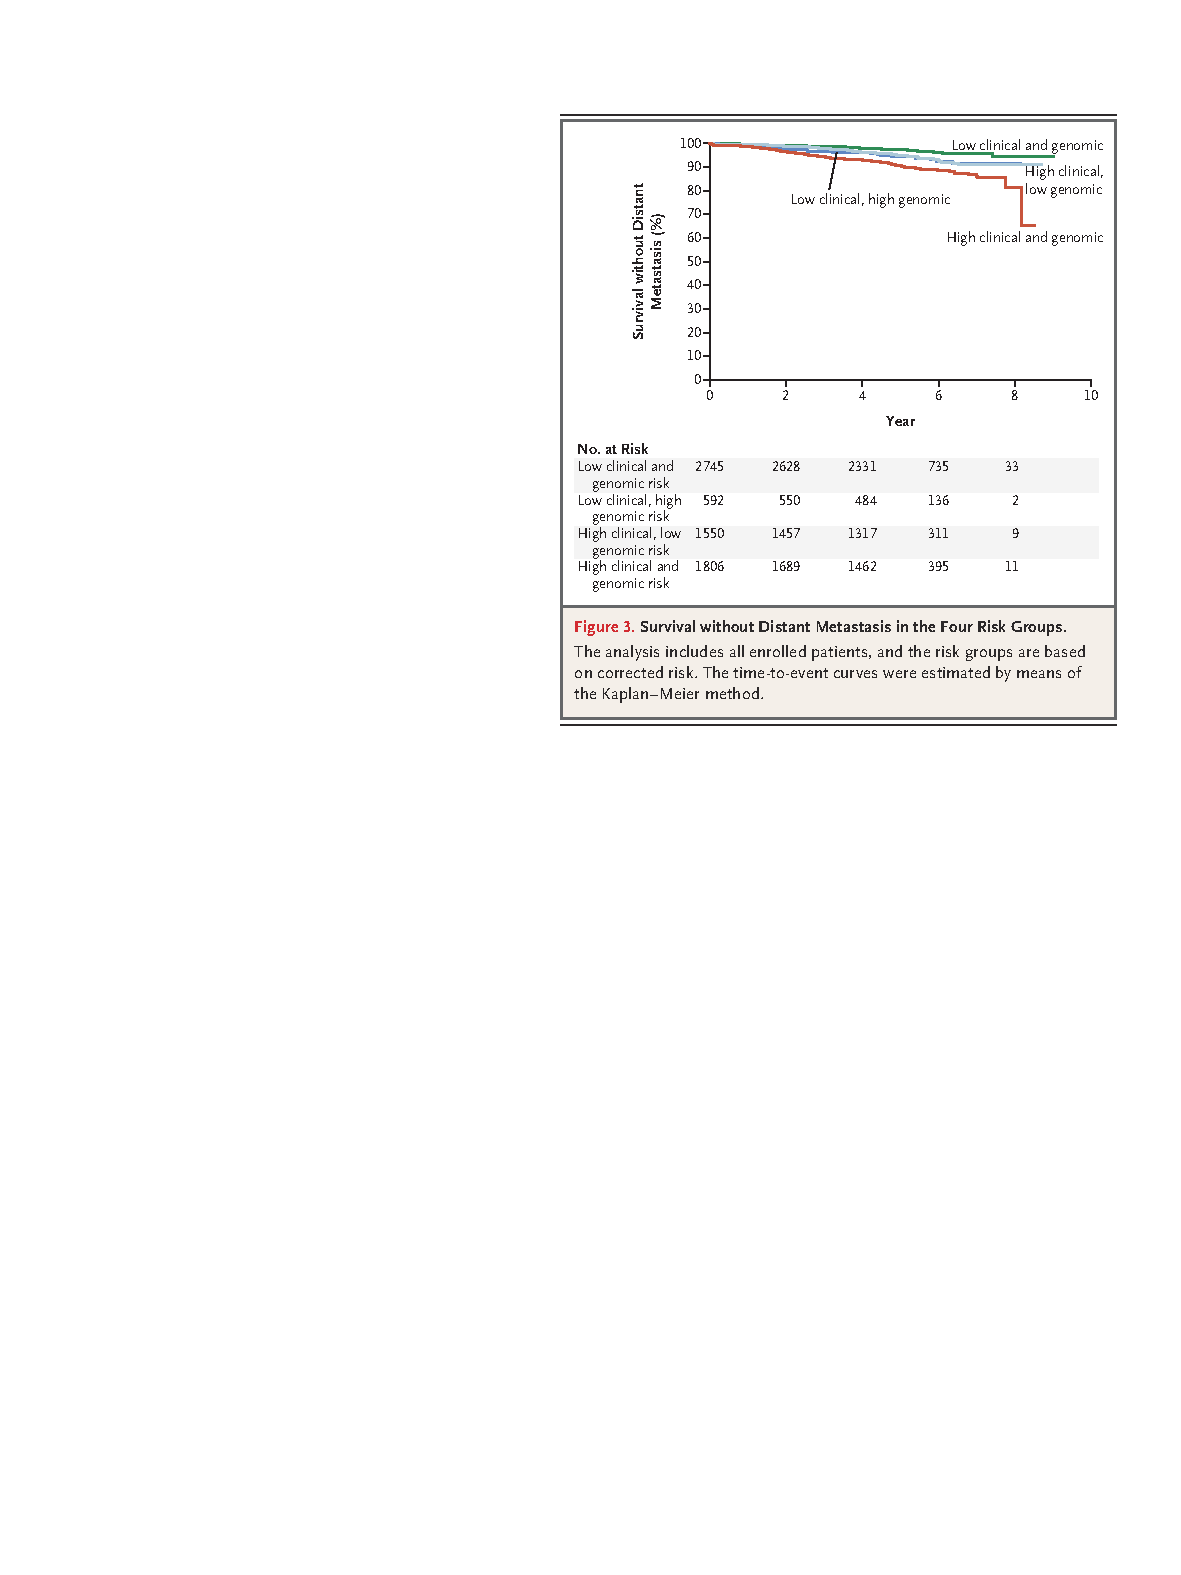
\includegraphics{figures/four_brca_groups.pdf}

\end{frame}

\begin{frame}{Time-to-event - Genomics and Breast Cancer, 25 Aug NEJM}

Confidence intervals for outcome: High clinical, low genomic risk:

\begin{itemize}
\item
  No chemo: 5-yr estimate: (92.5\%, 96.2\%)
\item
  Hazard ratio, chemo vs no-chemo: (0.5, 1.21), p = 0.27
\end{itemize}

\vspace{-0.45in}

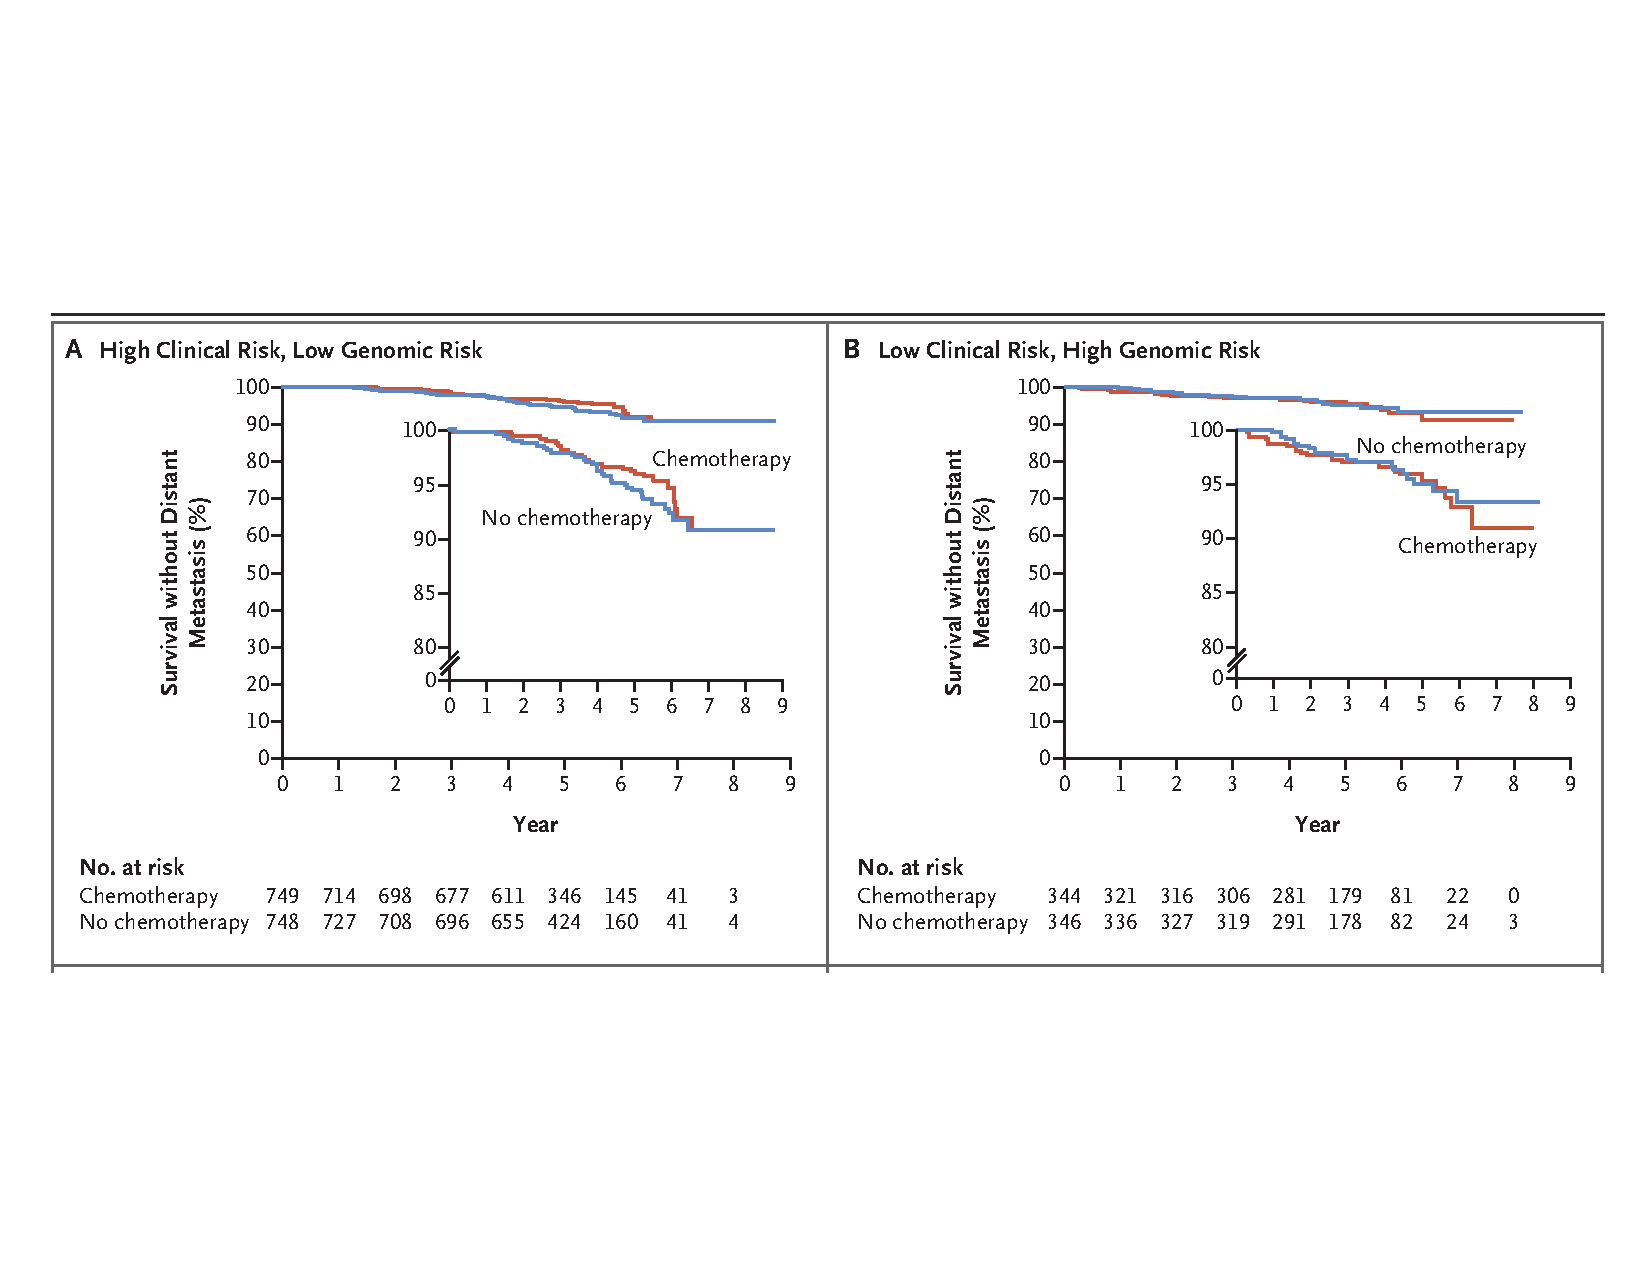
\includegraphics{figures/surv_wo_mets.pdf}

\end{frame}

\begin{frame}{Time-to-event outcomes - SPRINT}

Cumulative hazards and hazard ratio

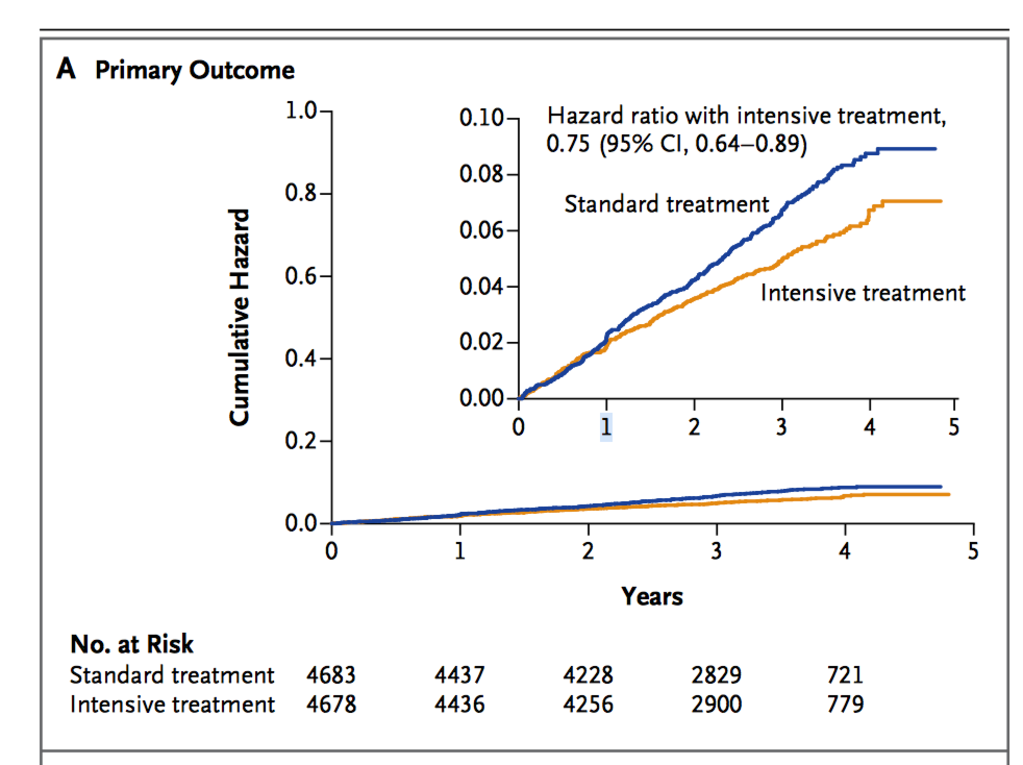
\includegraphics{figures/sprint_primary_outcome.pdf}

\end{frame}

\section{Confounding in observational
studies}\label{confounding-in-observational-studies}

\begin{frame}{East Boston study of adolescents}

Data from a study examining lung function in 654 children from East
Boston.

Among many variables, study recorded

\begin{itemize}
\item
  Age
\item
  Smoking status (yes/no)
\item
  Lung function, forced expiratory volume of air expelled in 1 second
  (fev)

  \begin{itemize}
  \itemsep1pt\parskip0pt\parsep0pt
  \item
    Measured in liters
  \end{itemize}
\end{itemize}

Tager, et. al \textit{Am J Epi}, 1979

\end{frame}

\begin{frame}{Association between lung function and smoking}

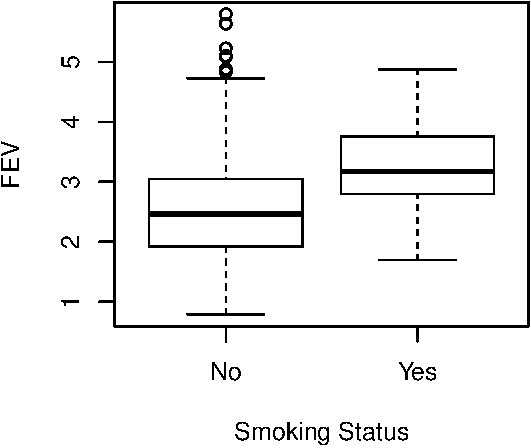
\includegraphics{reporter_course_harrington_files/figure-beamer/unnamed-chunk-1-1.pdf}\\

\end{frame}

\begin{frame}{Confounding}

Previous plot suggests that smoking is associated with an average
increase in lung function

\begin{itemize}
\itemsep1pt\parskip0pt\parsep0pt
\item
  Smokers have (on average) an FEV that is higher by 0.7 liters/sec
\end{itemize}

Association can be caused by confounding.

A confounding variable is

\begin{itemize}
\item
  Associated with outcome
\item
  Associated with exposure
\end{itemize}

Natural variable to examine here is age

\end{frame}

\begin{frame}{Adjusting for confounding}

We use statistical models to estimate the simultaneous association

\begin{itemize}
\item
  Age and smoking status with FEV.
\item
  Perhaps age, height and smoking status with FEV
\end{itemize}

If it works, it will show the association of smoking and FEV

\begin{itemize}
\itemsep1pt\parskip0pt\parsep0pt
\item
  After adjusting for age and height.
\end{itemize}

\end{frame}

\begin{frame}{Model based adjustments}

Association of smoking and FEV, after adjusting for

\begin{itemize}
\item
  age: decrease in FEV of approximately 0.30 liters/sec
\item
  age and height: decrease of approximately 0.10 liters/sec
\item
  age, height and age by height interaction: decrease of 0.17 liters/sec
\end{itemize}

Depending on model, estimated association varies

\begin{itemize}
\itemsep1pt\parskip0pt\parsep0pt
\item
  But all adjustments suggest smoking is associated with decrease in
  lung function
\end{itemize}

\end{frame}

\begin{frame}{Some caveats with model based adjustments}

Most datasets are far more complex than the East Boston study

We have no way of knowing which adjustment is correct

\begin{itemize}
\itemsep1pt\parskip0pt\parsep0pt
\item
  Specific numerical values of adjusted associations less important than
  direction.
\end{itemize}

Statisticians discourage the use of the phrase

\begin{itemize}
\itemsep1pt\parskip0pt\parsep0pt
\item
  `Association of smoking and fev, after \emph{controlling} for
  \ldots{}'
\end{itemize}

Watch out for implied causal claims

\end{frame}

\begin{frame}{Other ways to adjust for confounders}

Analyse separately by subgroups (stratify)

Match each smoker with a nonsmoker with similar age and height
(matching)

\begin{itemize}
\itemsep1pt\parskip0pt\parsep0pt
\item
  Requires a large dataset, difficult to do if it matching was not built
  into the design
\end{itemize}

Create a model for the probability of smoking, given participant
characteristics

\begin{itemize}
\item
  The match smokers, nonsmokers with similar probabilities
\item
  Called propensity score matching
\end{itemize}

All approaches less reliable when there are unmeasured confounders.

\end{frame}

\section{Closing out}\label{closing-out}

\begin{frame}{These points bear repeating}

We do not expect designs or analyses to be perfect

We look for

\begin{itemize}
\item
  Transparency
\item
  Following principles of scientific investigations: formulating a
  hypothesis, then testing it
\item
  Use of `state of the practice' methods
\item
  Sensitivity analyses: do different models lead to the same qualitative
  conclusion
\end{itemize}

\end{frame}

\end{document}
